\documentclass[14pt]{extarticle}
\usepackage{fontspec}
\usepackage{polyglossia} % use instead of babel
\usepackage{pgfplots}
\usepackage{float}
\usepackage{amsmath}
\setdefaultlanguage{hebrew}
\setotherlanguage{english}
\newfontfamily\hebrewfont[Script=Hebrew]{Arial}

% TODO: figure out if better to keep this or not, for word document pdf output similarity
\usepackage[margin=1in]{geometry}

% might be useful to ensure similarity to word document pdf output
% \usepackage{setspace}
% \singlespacing

% Reset equation counter at the start of each section
\usepackage{chngcntr}
\usepackage{etoolbox}
\counterwithin*{equation}{section}
\preto{\section}{\setcounter{equation}{0}}

\begin{document}

\begin{center}
    {\LARGE \textbf{ממ"ן 13}}\\
    {\textbf{חוקי ניוטון}}
\end{center}

\begin{itemize}
    \item מגישים: תומר רוזנפלד, שי רואימי
    \item תאריך ביצוע הניסוי: 28 יולי 2025
    \item מדריך הניסוי: ד"ר סילביו ריינהורן
\end{itemize}
\newpage

\section*{ניסוי 1 - החוק הראשון של ניוטיון}
\subsection*{מטרת הניסוי}
בדיקת תוקפו של החוק הראשון של ניוטון
\subsection*{רקע תיאורטי}
החוק הראשון של ניוטון קובע כי גוף ששקול הכוחות עליו הוא אפס נשאר מתמיד במצב מנוחה או בתנועה במהירות קבועה בקו ישר.

בנוסף, מיקום גוף ביחס לזמן מתואר ע"י המשוואה:
\begin{equation}
x(t) = x_0 + v_0 t + \frac{1}{2} a t^2
\end{equation}
כאשר $x(t)$ הוא מיקום הגוף ביחס לזמן, $x_0$ הוא מיקום הגוף בהתחלת המדידה, $v_0$ היא מהירות הגוף בהתחלת המדידה, $a$ היא תאוצת הגוף ו-$t$ הוא הזמן שחלף מאז התחלת המדידה.

\subsection*{מערכת המדידה ומהלך הניסוי}
ראשית איזנו מסילה כך שהייתה אופקית לחלוטין. בדקנו את אופקיות המסילה ע"י הנחת עגלה במקומות שונים על המסילה וראינו שהיא נשארה במקום.  בנוסף בדקנו בעזרת פלס.

בקצה של המסילה חיברנו חיישן תנועה, בניסוי זה  נעזרנו בו למדידת מיקום העגלה.

לאחר מכן דחפנו קלות את העגלה והקלטנו את תוצאות המדידה בתוכנת PASCO Capstone. המדידה הכילה את מיקום העגלה ביחס לזמן התחלת ההקלטה.

\subsection*{תוצאות וניתוח}
הגרף הבא מציג את מיקום העגלה ביחס לזמן: 
\begin{figure}[H]
    \centering
    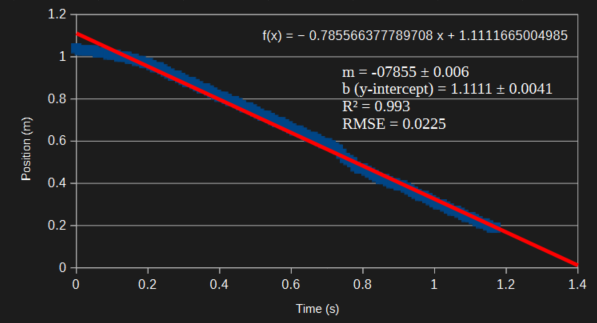
\includegraphics[width=0.8\textwidth]{maman_13_experiment_1_position_time_graph.png}
    \caption{מיקום העגלה ביחס לזמן}
\end{figure}

ניתן לראות שהגרף מתואר היטב ע"י פונקציה ליניארית עם שיפוע $m=0.7856$ ולכן ע"י הצבה במשוואה 1:
\begin{center}
\begin{equation}
\begin{aligned}
    x(t) &= x_0 + v_0 t + \frac{1}{2} a t^2 \\
    x_0 &= 1.1111 \\
    a &= 0 \\
    v_0 &\equiv \textbf{שיפוע הגרף} = -0.7856 \\
\end{aligned}
\end{equation}
\end{center}
סימן המינוס הוא מכיוון שכיוון התנועה של העגלה הוא לכיוון חיישן התנועה.
כיוון והגרף מתואר ע"י פונקציה ליניארית אין תלות ב $t^2$, כלומר התאוצה $a=0$, וכן $x_0 = 1.1111$ הוא מיקום העגלה בהתחלת המדידה.

\subsection*{דיון ומסקנות}
בניסוי שקול הכוחות על הגוף בציר התנועה (המסילה) היה אפס וכך יכלנו לבדוק את קיום החוק הראשון של ניוטון.

במדידה קיבלנו גרף מקום ביחס לזמן, עם התאמה טובה לפונקציה ליניארית,  ומשם הסקנו כי מהירות הגוף קבועה - כלומר הגוף מתמיד במצב תנועה במהירות קבועה בקו ישר, כפי שקובע החוק הראשון של ניוטון.

החוסר התאמה הליניארית בגרף יכולה לנבוע מחיכוך, כאשר החיכוך עלול להשתנות גם כתלות במיקום הגוף על המסילה (המסילה אינה חלקה לכל אורכה), וגם אולי משיפוע קל במסילה.

בניסוי זה לא היה ניתן לחשב שגיאת מדידה כיוון שהמהירות ההתחלתית ניתנה ע"י דחיפה קלה של העגלה, ולא נמדדה ישירות,  אבל יש לציין כי חוסר ההתאמה הליניארית בגרף עלולה לנבוע מחוסר איזון המסילה, חיכוך בין העגלה למסילה וכן שגיאת מדידה של החיישן.

\section*{ניסוי 2 - החוק השני של ניוטון - מסילה משופעת}
\subsection*{מטרת הניסוי}
חקירת תנועת עגלה במישור שיפוע ומדידת תאוצת הכובד

\subsection*{רקע תיאורטי}
בניסוי זה תנועת העגלה היא בשיפוע, ולכן נדרשים להתייחס לשקול הכוחות בציר האנכי וכן בציר האופקי.

הכוחות הפועלים על העגלה הם כוח הכבידה $F_g$, כוח נורמלי $F_n$ וכוח חיכוך $F_f$.
כוח הכבידה פועל כלפי מטה, וכוח החיכוך כנגד כיוון התנועה. בניסוי זה נתעלם מכוח החיכוך בחישובים.

האיור הבא מתאר את הכוחות הפועלים על העגלה, כאשר כוח החיכוך לא מצויין, והוא כנגד כיוון התנועה:
\begin{figure}[H]
    \centering
    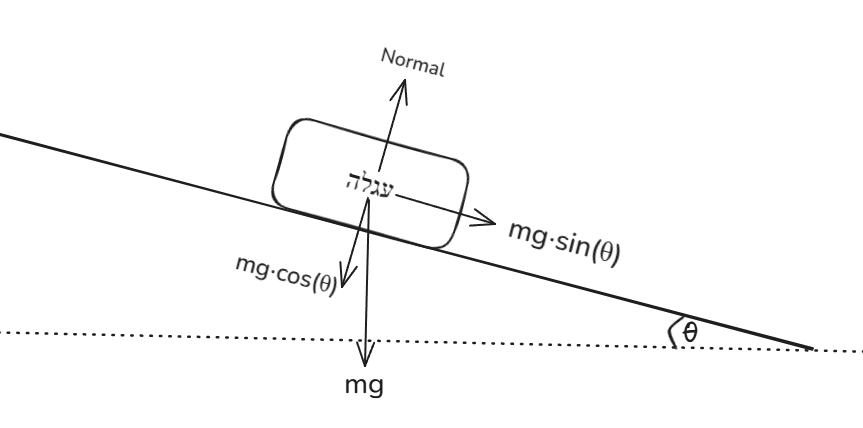
\includegraphics[width=0.5\textwidth]{maman_13_experiment_2_forces_chart.png}
    \caption{כוחות הפועלים על העגלה}
\end{figure}

נתייחס לציר המקביל למסילה כציר ה-x, כידוע, ע"פ החוק השני שני של ניטון:
\begin{center}
\begin{equation}
\begin{aligned}
\Sigma F & = m a \\
F_x & = m a_x = mg \sin(\theta)
\end{aligned}
\end{equation}
\end{center}

\subsection*{מערכת המדידה ומהלך הניסוי}
בניסוי זה הרכבנו עגלה על מסילה משופעת. את השיפוע מדדנו בעזרת מד זווית. בקצה המסילה הרכבנו חיישן תנועה.

בחלק הראשון של הניסוי שחררנו את העגלה ממרחק 60 ס"מ מהחיישן, כאשר המסילה בזווית 4 מעלות.
בעזרת חיישן התנועה מדדנו את מיקום העגלה ביחס לזמן, והקלטנו את תוצאות המדידה בתוכנת PASCO Capstone

לאחר מכן ביצענו את אותה מדידה, כאשר הנחנו משקולת על העגלה.

בחלק השלישי של הניסוי מדדנו את תאוצת העגלה בירידה בזוויות שונות ($\theta = 4^\circ, 5^\circ, 6^\circ, 7^\circ, 8^\circ$).
בעזרת התוצאות מהמדידה חישבנו את תאוצת הכובד $g$.

\subsection*{תוצאות וניתוח}
כאמור, בחלק הראשון של הניסוי שיחררנו את העגלה ממרחק 60 ס"מ מהחיישן, כאשר המסילה בזווית 4 מעלות.
המדידה כוללת את הירידה של העגלה, וכן את העלייה חזרה עד שיא הגובה.

הגרף הבא מציג את מיקום העגלה ביחס לזמן, כאשר ציר ה-y המסומן בתור Position
מתאר את המרחק מחיישן התנועה:
\begin{figure}[H]
    \centering
    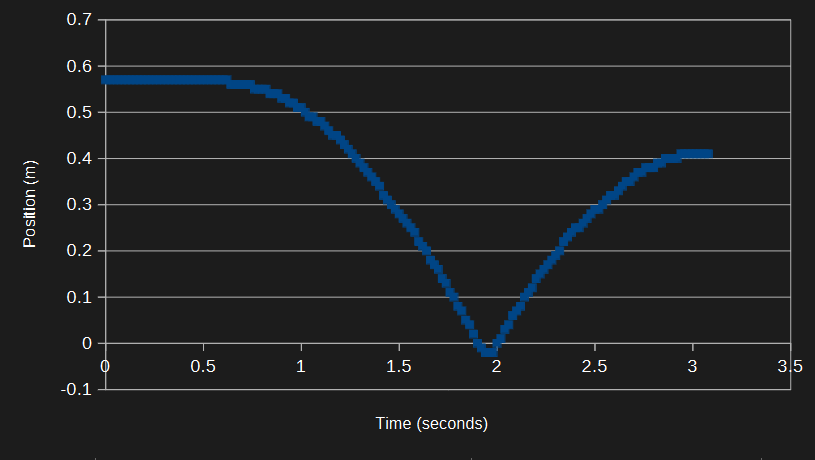
\includegraphics[width=0.8\textwidth]{maman_13_experiment_2_position_time_4_degrees_no_weight.png}
    \caption{מיקום העגלה ביחס לזמן}
\end{figure}

ניתן לראות מהגרף שלאחר שחרור העגלה, העגלה היא יורדת במהירות שגדלה עם הזמן, כלומר התאוצה חיובית.
בערך בשנייה השנייה לתנועה העגלה מגיעה לקפיץ וכיוון המהירות מתהפך. בחלק זה של התנועה המהירות הולכת וקטנה עד שהעגלה מגיעה לשיא הגובה, שם היא מתאפסת. 
לאורך כל התנועה התאוצה קבועה, וכיוונה כלפי מטה (כלפי חיישן התנועה).

העגלה התחילה במיקום 60 ס"מ מהחיישן, ובסוף התנועה נעצרה במרחק 40 ס"מ.
מכך אפשר ללמוד, כפי שאמרנו קודם, שהתאוצה לכיוון מטה (לכיוון חיישן התנועה) ולכן המהירות בעלייה מתאפסת לפני חזרת העגלה ל 60 ס"מ.

באותה מדידה, החיישן גם מדד את מהירות העגלה ביחס לזמן. נחלק את המדידה לשני גרפים, עלייה וירידה:

\begin{figure}[H]
    \centering
    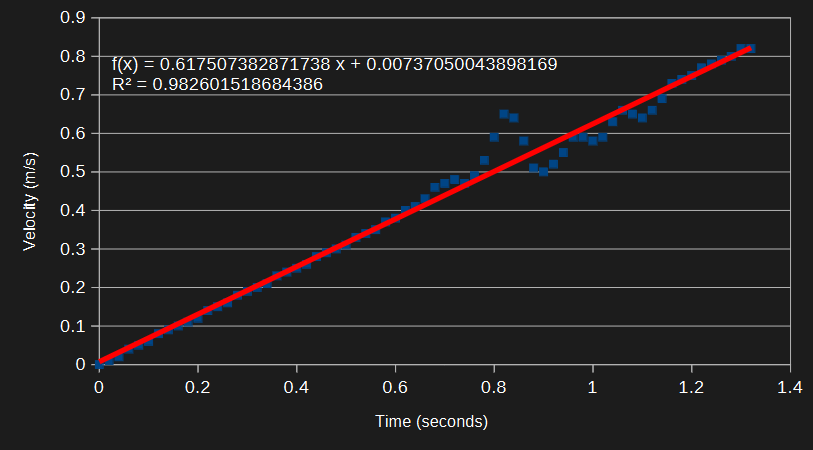
\includegraphics[width=0.8\textwidth]{maman_13_experiment_2_4_deg_no_weight_velocity_to_time_downhill.png}
    \caption{מהירות העגלה ביחס לזמן בירידה}
\end{figure}

\begin{figure}[H]
    \centering
    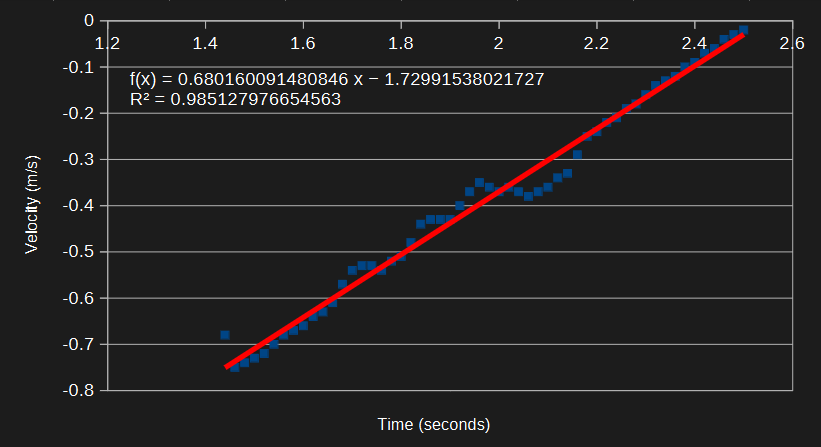
\includegraphics[width=0.8\textwidth]{maman_13_experiment_2_4_deg_no_weight_velocity_to_time_uphill.png}
    \caption{מהירות העגלה ביחס לזמן בעלייה}
\end{figure}

ע"פ הגרף המהירות המרבית של העגלה היא 0.8 מטר לשנייה, כאשר העגלה ממש לפני הפגיעה בקפיץ בסוף הירידה.
בשיא הגובה כמובן שהעגלה מגיעה לעצירה רגעית ולכן מהירות העגלה היא אפס.

ניתן למצוא את התאוצה בעלייה ובירידה ע"י התאמה ליניארית בגרף, כאשר התאוצה שווה לשיפוע הגרף.

בירידה התאוצה היא $0.6175 \frac{m}{s^2}$, ובעלייה התאוצה היא $0.6801 \frac{m}{s^2}$. כפי שהסברנו ברקע התיאורטי קיים בניסוי זה גם כוח חיכוך שפועל נגד כיוון התנועה.
הכוח שמפעיל כוח המשיכה לכיוון החיישן ($mg \sin(\theta)$) קבוע.
 בנוסף אליו, בירידה כוח החיכוך פועל לכיוון מעלה, ואילו בעלייה  כוח החיכוך פועל כלפי מטה.

 כלומר בירידה הכוחות הללו מנוגדים בכיוונם ובעלייה הם פועלים לאותו כיוון (מטה), ולכן התאוצה בעלייה גדולה יותר מהתאוצה בירידה.

 בחלק הבא של הניסוי התבקשנו לעשות את אותה מדידה כאשר הנחנו משקולת על העגלה.
 מצ"ב הגרפים של מהירות העגלה ביחס לזמן בירידה ובעלייה, כאשר העגלה נושאת משקולת של 100 גרם:
\begin{figure}[H]
    \centering
    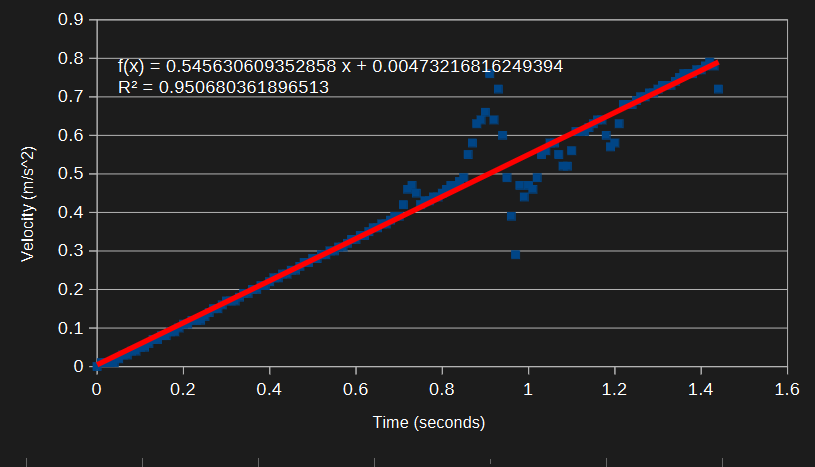
\includegraphics[width=0.8\textwidth]{maman_13_experiment_2_4_deg_weighted_velocity_to_time_downhill.png}
    \caption{מהירות העגלה ביחס לזמן בירידה עם משקולת}
\end{figure}        

\begin{figure}[H]
    \centering
    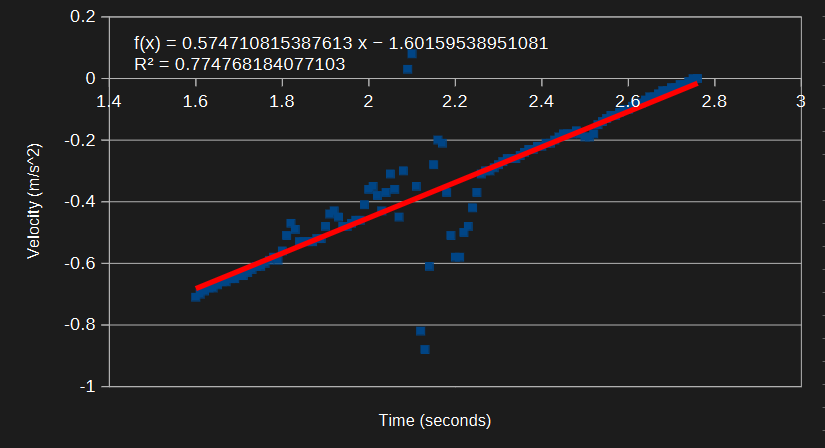
\includegraphics[width=0.8\textwidth]{maman_13_experiment_2_4_deg_weighted_velocity_to_time_uphill.png}
    \caption{מהירות העגלה ביחס לזמן בעלייה עם משקולת}
\end{figure}

התאוצה בירידה עם משקל היא $0.5456 \frac{m}{s^2}$ ובעלייה עם משקל היא $0.5747 \frac{m}{s^2}$.
לפי חוקי ניוטון:,
\begin{equation}
\begin{aligned}
F_{gravity} &= m g \sin(\theta) \\
F_{friction} &= \mu m g \cos(\theta) \\
F_{net} &= F_{gravity} - F_{friction} \\
a &= \frac{F_{net}}{m} = g \sin(\theta) - \mu g \cos(\theta)
\end{aligned}
\end{equation}
כלומר, בתיאוריה התאוצה אינה תלויה במסה. אבל בפועל בתנועה עם גלגלים החיכוך הרלוונטי הוא
\textbf{חיכוך התגלגלות},
שערכו: $F_{rolling} = c_r N$,
כאשר
$c_r$
הוא מקדם חיכוך התגלגלות, ויכול לגדול עם המסה, ו-
$N$
הוא הכוח הנורמלי.

בחלק האחרון של הניסוי מדדנו את תאוצת העגלה בזוויות שונות, בירידה בלבד:
\begin{table}[H]
    \centering
    \begin{tabular}{|c|c|c|}
        \hline
        זווית ($\theta$) & תאוצה ($a$) [$\frac{m}{s^2}$] & $\sin(\theta)$ \\
        \hline
        $4^\circ$ & 0.643 & 0.0697 \\
        $5^\circ$ & 0.799 & 0.0871 \\
        $6^\circ$ & 0.978 & 0.1045 \\
        $7^\circ$ & 1.14 & 0.1219 \\
        $8^\circ$ & 1.38 & 0.1392 \\
        \hline
    \end{tabular}
    \caption{תאוצת העגלה בזוויות שונות}
\end{table}

מהטבלה ייצרנו גרף של תאוצת העגלה כתלות בסינוס זווית ההטיה:

\begin{figure}[H]
    \centering
    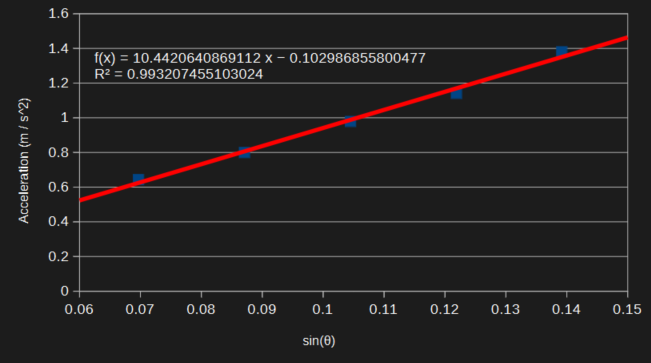
\includegraphics[width=0.8\textwidth]{maman_13_experiment_2_acceleration_to_sin_degrees_graph.png}
    \caption{תאוצת העגלה כתלות בסינוס זווית ההטיה}
\end{figure}

אם נתעלם מכוח החיכוך נקבל:
\begin{equation}
\Sigma F = m a = m g \sin(\theta) \Rightarrow a = g \sin(\theta)
\end{equation}

כלומר, שיפוע הגרף שווה לתאוצת הכובד $g$.
השיפוע ההתקבל הוא:
\begin{equation}
\text{שיפוע} = 10.44 \Rightarrow g = 10.44 \frac{m}{s^2}
\end{equation}

\subsection*{דיון ומסקנות}
בחלק הראשון של הניסוי בחנו את תנועת העגלה בנפילה במדרון משופע לפני ואחרי פגיעה בקפיץ.
הסתכלנו על מיקום העגלה ומהירות העגלה ביחס לזמן,
וראינו כי התאוצה קבועה (בכל חלק בתנועה) וכיוונה כלפי מטה, כלומר כיוון חיישן התנועה.
בנוסף, ראינו שהעגלה לא חזרה לגובהה ההתחלתי, זאת כתוצאה מחיכוך, וכן מהתנגדות הקפיץ.

בחלק השני של הניסוי ראינו את ההשפעה של הוספת משקל לעגלה. ראינו את התאוצה יורדת, וזאת כתוצאה מהתנגדות חיכוך התגלגלות, שגדלה עם המסה.

ובחלק האחרון בחנו את תאוצת העגלה בנפילה מזוויות שונות, ובעזרת המדידות והתאמה ליניארית הצלחנו למצוא את קבוע הכבידה $g$.

כמובן שהערך הידוע בספרות הוא $g = 9.81 \frac{m}{s^2}$, והשגיאה היחסית היא:
\begin{equation}
\text{שגיאה יחסית} = \frac{10.44 - 9.81}{9.81} \approx 6.42\%
\end{equation}

\section*{ניסוי 3 - החוק השני של ניוטון - כוח  חופשי}
\subsection*{מטרת הניסוי}
מציאת מסת עגלה בעזרת הפעלת כוח חופשי
\subsection*{רקע תיאורטי}   
כידוע, ע"פ החוק השני שני של ניטון:
\begin{equation}
\Sigma F = m a
\end{equation}
כאשר $\Sigma F$ הוא סכום הכוחות הפועלים על גוף, $m$ היא מסת הגוף ו-$a$ היא תאוצת הגוף.
ניסוי זה מתרחש על מסילה מאוזנת, כך שנתייחס ררק לכוחות בציר האופקי.
וכן בציר האופקי הכוח המרכזי הפועל הוא הכוח שנפעיל בעת דחיפת ומשיכה העגלה ובכן

\begin{equation}
F_{push} = m a
\end{equation}
\subsection*{מערכת המדידה ומהלך הניסוי}
על  מסילה מ אוזנת הרכבנו עגלה וחיישן כוח המחובר לעגלה.
תפסנו בוו של  חיישן הכוח עם היד ודחפנו את העגלה מצד לצד, כאשר במקביל מדדנו  את הכוח והתאוצה  ביחס לזמן (בעזרת החיישן).
\subsection*{תוצאות וניתוח}
הגרף הבא מציג את הכוח ביחס לזמן:
\begin{figure}[H]
    \centering
    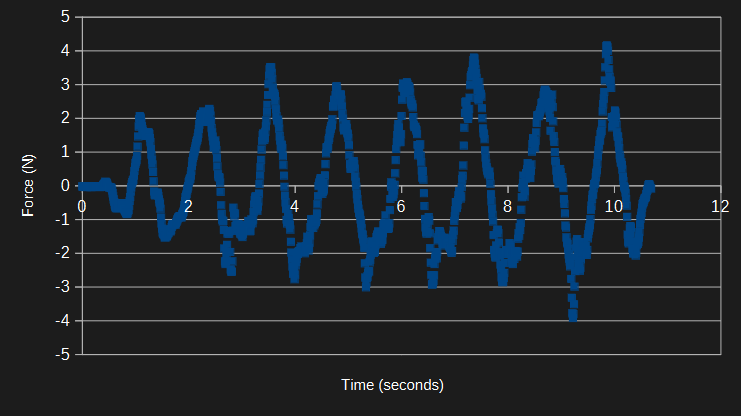
\includegraphics[width=0.8\textwidth]{maman_13_experiment_3_force_to_time.png}
    \caption{כוח ביחס לזמן}
\end{figure}
והגרף הבא מציג את התאוצה ביחס לזמן:
\begin{figure}[H]
    \centering
    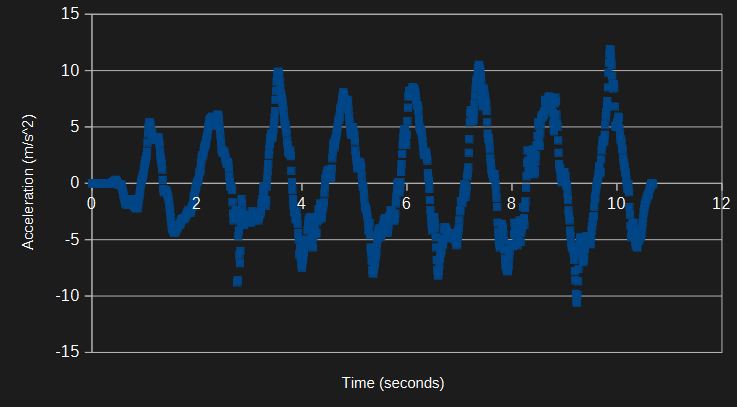
\includegraphics[width=0.8\textwidth]{maman_13_experiment_3_acceleration_to_time.png}
    \caption{תאוצה ביחס לזמן}
\end{figure}

ניתן לראות שכיוון התאוצה וכיוון הכוח משתנים יחד, כפי שציפינו ע"פ החוק השני של ניוטון.
כיוון התאוצה והכוח מתבטא בחיוביות או שליליות הערכים בגרף. כלומר, כאשר העגלה נעה ימינה הכוח והתאוצה חיוביים, וכאשר העגלה נעה שמאלה הכוח והתאוצה שליליים.

הנקודות בהן הכוח והתאוצה שווים לאפס מתארות את הרגע בו העגלה מפסיקה לנועה  לכיוון אחד ומתחילה לנוע לכיוון השני.

ונקודות הקיצון בגרף הכוח מתארות את הרגע בו הכוח המופעל על העגלה הוא מקסימלי באותה דחיפה או משיכה, כלומר הרגע בו הדחיפה או המשיכה של העגלה היא החזקה ביותר, ובהתאם לכך התאוצה היא מקסימלית.

בהמשך ניסוי התבקשנו לייצר גרף של כוח ביחס לתאוצה, כלומר לגרף הבא:
\begin{figure}[H]
    \centering
    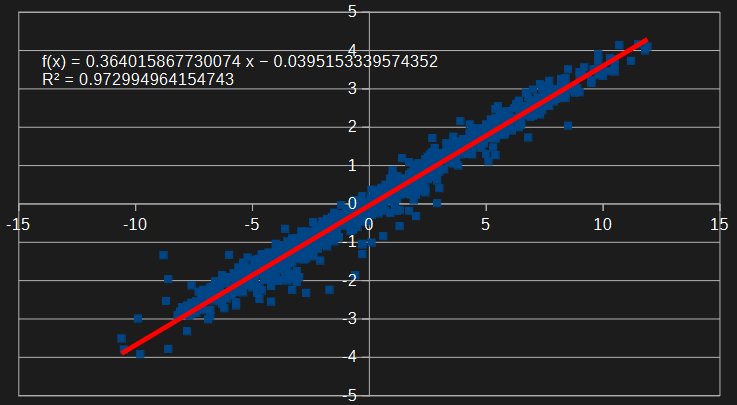
\includegraphics[width=0.8\textwidth]{maman_13_experiment_3_force_to_acceleration.png}
    \caption{כוח ביחס לתאוצה}
\end{figure}

ע"פ נוסחא 2 בסעיף זה, ניתן לייצג את הקשר $m = \frac{F_{push}}{a}$, כלומר שיפוע הגרף הוא מסת העגלה.
את שיפוע מצאנו ע"י התאמה ליניארית וערכו 0.364, כלומר ע"פ המדידה מסת העגלה היא 364 גרם.

שקילת העגלה במשקל החזירה את הערך 355.9 גרם.

\subsection*{דיון ומסקנות}
שקילת העגלה במשקל החזירה את הערך 355.9 גרם, כלומר השגיאה היחסית היא:
\begin{equation}
\text{שגיאה יחסית} = \frac{364 - 355.9}{355.9} \approx 2.7\%
\end{equation}
שגיאה זו עלולה לנבוע כתוצאה מהתעלמות מכוח החיכוך של העגלה במסילה, וכן משגיאה במדידת הכוח או התאוצה.

ההתעלמות מכוח החיכוך מתבטאת במעבר ממשוואה 1 למשוואה 2 בסעיף זה, כאשר קבענו כי $\Sigma F = F_{push}$, כלומר התעלמנו מכוח החיכוך שגם פועל בציר האופקי.

בניסוי זה מדדנו את הכוח המופעל על העגלה ואת התאוצה בעזרת חיישן, וע"י הנתונים שנאספו הצלחנו להראות את היחס הישר בין הכוח המופעל על העגלה לבין התאוצה שלה, וכן למצוא בקירוב את מסת העגלה, ובכך להראות את קיומו של החוק השני של ניוטון.

\end{document}